% 3. Equivalent Cashflow Equestions
% Stu Alden
%----------------------------------------------------------------------------------------

\documentclass[14pt]{extarticle}

\usepackage{conceptsheet}

%---------------------------------------
\begin{document}

\finmathtitle{3. Equivalent Cashflow Equations}

Different cashflows can be compared and equated, at a particular compound interest rate, by
accumulating and/or discounting all flows to a single ``measurement'' or ``comparison'' date.

We've already been doing this---for example, when you get a future value and need to calculate a
present value, or vice versa.  But we can have any kind of combination of \textbf{multiple} cash
flows, both positive and negative, with any kind of timing, and the basic process still works.

One particularly nice aspect of compound interest is that you get the same equivalence results
\underline{regardless of your choice of comparison date}.

\vspace{.2in}
\textbf{An Example:}

Let's say you borrow \$100 today, and you plan to repay the loan with \$50 6 months from now and the rest a year
from now.  If the interest rate is 6\% compounded monthly, how much is that second payment?

We start by drawing a timeline, putting what we know in the appropriate places:

\begin{center}
  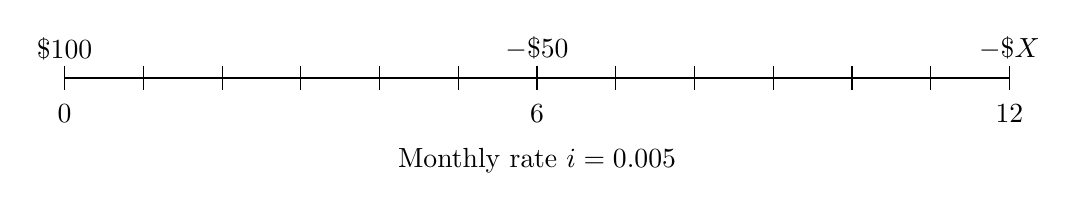
\begin{tikzpicture}[scale=1]

    % Main horizontal axis
    \draw[thick] (0,0) -- (12,0);

    % Tick marks
    \foreach \x in {0,...,12}
    \draw (\x,0.15) -- (\x,-0.15);

    % Amounts above exis
    % Month labels below axis
    \draw (0,0) node[below=6pt] {$ 0 $} node[above=3pt] {$ \$100 $};
    \draw (6,0) node[below=6pt] {$ 6 $} node[above=3pt] {$ -\$50 $};
    \draw (12,0) node[below=6pt] {$ 12 $} node[above=3pt] {$ -\$X $};

    % Monthly rate label below
    \node[below=22pt] at (6,0)
    {Monthly rate $i = 0.005$};

    % Vertical accumulation factors
    % \foreach \x in {1,...,12}
    % \node[
    %   rotate=90,
    %   anchor=base,
    %   font=\scriptsize
    % ] at (\x+0.08,0.85)
    % {$ (1.005)^{\x} $};

  \end{tikzpicture}
\end{center}

We are showing the \$100 as positive (what you borrowed) and the other values as negative (what you pay back).

Next, pick a convenient measurement date.  A good choice for this problem would be time 0, so the \$100 needs
no adjustment.  We just need to ``bring back'' the \$50 by 6 months and the \$X by one year:

\[
  100 = 50(1 + 0.005)^{-6} + X(1+.005)^{-12}
\]

Solving for X, we get \$54.65, the amount that must be repaid at the end of the year.

\pagebreak
%\vspace{.2in}
\textbf{Notes:}

\begin{itemize}

  \item If we maintain the sign convention for each payment (whether it's a payment from you or to you), we can simply add
    up all payments (with the appropriate payment timing adjustment for interest) and set the signed sum of all payments to
    zero.

  \item This equation approach works for any variable, not just payments.  For example, you might instead be solving for
    the time at which a payment must be made, or for the interest rate in effect.

\end{itemize}


\end{document}
